\documentclass[twoside,12pt,a4paper,titlepage]{article}

\usepackage{xspace}
\usepackage{siunitx}
\usepackage{booktabs}
\usepackage{rotating}
\usepackage[margin=2.5cm]{geometry}

\newcommand{\org}{The Smallpeice Trust\xspace}
\newcommand{\staff}{Smallpeice Trust staff and volunteers\xspace}
\newcommand{\gamename}{Tin Can Rally\xspace}
\newcommand{\timeline}{August 2017\xspace}

\title{\gamename}
\author{\org}
\date{\timeline}

\usepackage{helvet}
\renewcommand{\familydefault}{\sfdefault}

\usepackage[pdftex,
            hidelinks]{hyperref}

\begin{document}

\begin{titlepage}
\begin{center}

\includegraphics[width=0.55\textwidth]{./soton_logo.eps}~\\[1cm]
\textsc{\large Electronics and Computer Science}\\[0.2cm]
\textsc{\large Faculty of Physical Sciences and Engineering}\\[0.2cm]
\textsc{\large University of Southampton}\\[3.5cm]

\includegraphics[width=0.55\textwidth]{./smallpeice_logo.jpg}~\\[1cm]
\textsc{\large The Smallpeice Trust}\\[3.5cm]
\textsc{\huge \textbf{\gamename{}: Rules}}\\[1cm]
\textsc{\large \timeline}\\[3cm]
\textsc{\Large Computing and Microelectronics}
\end{center}
\end{titlepage}

\section{Game Rules}
\label{sec:rules}

\begin{enumerate}
  \item The game, called \emph{\gamename}, is played in the arena defined in
        Specification~\ref{spec:arena}. The objective is to race around a
        track, picking up cans along the way.
  \item 3 points are awarded each time a robot crosses a track boundary in the
        anticlockwise direction.
  \item Robots can pick up tokens which are in the track. Each time a robot
        crosses a track boundary and is awarded a track boundary point, it is
        awarded 2 bonus points for each token it is carrying.
  \item At every sixth track boundary, that is, every lap, a robot is awarded
        an additional 2 points above the 3 for the crossing.
  \item At the end of a match, each robot is awarded 2 additional points for
        each token it is carrying.
  \item A robot is deemed to have passed a track boundary when the back of the
        robot passes the line.
  \item Cases of a robot passing backwards over a line are offset against
        future crossings forward of a line. That is, if a robot crosses two
        track boundaries backwards, it will need to cross two track boundaries
        forwards before it can gain any more track boundary points.
  \item Participating teams must present their robots to match officials at
        least one minute before the start of each match.
  \item There will be 2 robots in each match.
  \item \org may have any number of match officials within the arena, including
        during the course of matches.
  \item At the start of each match, robots must be entirely within their
        starting zones.
  \item At the start of each match, teams will be permitted to lean into the
        arena and start their robots.
  \item Each match lasts $120$ seconds.
  \item Teams may be disqualified from one or all matches by match officials,
        for non-compliance with regulations, lateness to the match, or any other
        reason at the discretion of the judge. Teams disqualified before the
        start time of a match will not be permitted to enter a robot.
\end{enumerate}


\clearpage
\section{Regulations}
\label{sec:regs}

\begin{enumerate}
\item The Judge's decision is final.
\item All robots must be safe.
  \begin{enumerate}
    \item This is defined considering safety concerns including, but not limited
          to:
      \begin{enumerate}
        \item sharp edges;
        \item the effects of impact at speed;
        \item fire risks from the battery (see Regulation~\ref{reg:lipo}).
      \end{enumerate}
    \item No robots will be permitted to compete without passing a safety and
          compliance inspection.
    \item \staff may reinspect your robot and invalidate previous inspections at
          any time.
  \end{enumerate}
\item Any assistance from \staff is provided without guarantees.
\item Competitors are expected to behave within the spirit of good
      sportsmanship.
\item Competitors must take reasonable measures to avoid their robot damaging
      the arena, or anything within it, including other robots. This is a
      non-contact sport.
\item Competitors are not permitted in the arena during the competition,
      except to lean in to start robots or where directed by match officials.
\item All robots must be fully autonomous once started. No remote control
      systems are permitted.
\item If you request your robot be turned off by marshals, you will be
      disqualified from that match.
\item At the start of each match, all competing robots must fit within a cube
      with edges of length \SI{500}{mm}. Expansion beyond this limit during the
      course of a match is permitted.
\item \label{reg:lipo}
      The Lithium-Polymer battery is the most dangerous part of the electronics
      kit and must be treated accordingly. Whenever a robot is in operation
      its battery must be:
  \begin{enumerate}
    \item securely held in place;
    \item adequately protected from damage even in the presence of damage to the
          rest of the robot;
    \item connected only to the main input of the power board.
  \end{enumerate}
%\item Additional batteries or other energy storage must be explicitly and
%      individually approved by \org before use.
\item A robot's main power switch must be easily accessible and on the top of
      the robot whenever the robot is powered.
\item A spare USB port to be used for competition control must be easily accessible.
%\item All robots must have badge mountings as described in
%      Specification~\ref{spec:badges}.
\item All electronics on a robot must be:
  \begin{enumerate}
    \item securely held in place;
    \item easily removable.
  \end{enumerate}

\item A robot must not have any devices designed to make sound, other
      than where provided directly by \org{}.
\end{enumerate}

\clearpage
\section{Specifications}
\label{sec:specs}
\newcounter{SpecID}

\subsection{Arena}
\refstepcounter{SpecID}
\label{spec:arena}

\begin{enumerate}
  \item The arena floor is a \SI{6}{m} $\times$ \SI{12}{m} rectangle.
  \item The layout of the arena is given in Figure~\ref{fig:arena}. This
        figure is to scale.
  \item The docking area is \SI{1.5}{m} $\times$ \SI{1.5}{m}.
  \item The raised areas are each \SI{1.5}{m} $\times$ \SI{1}{m}, and raised
        from the floor by \SI{0.5}{m}.
  \item The starting zones are centrally aligned, share one side with the
        north wall of the arena, and are \SI{0.9}{m} $\times$ \SI{0.9}{m}.
  \item The canonical definition of the arena is what is in the simulator.
\end{enumerate}

\begin{figure}
  \centering
  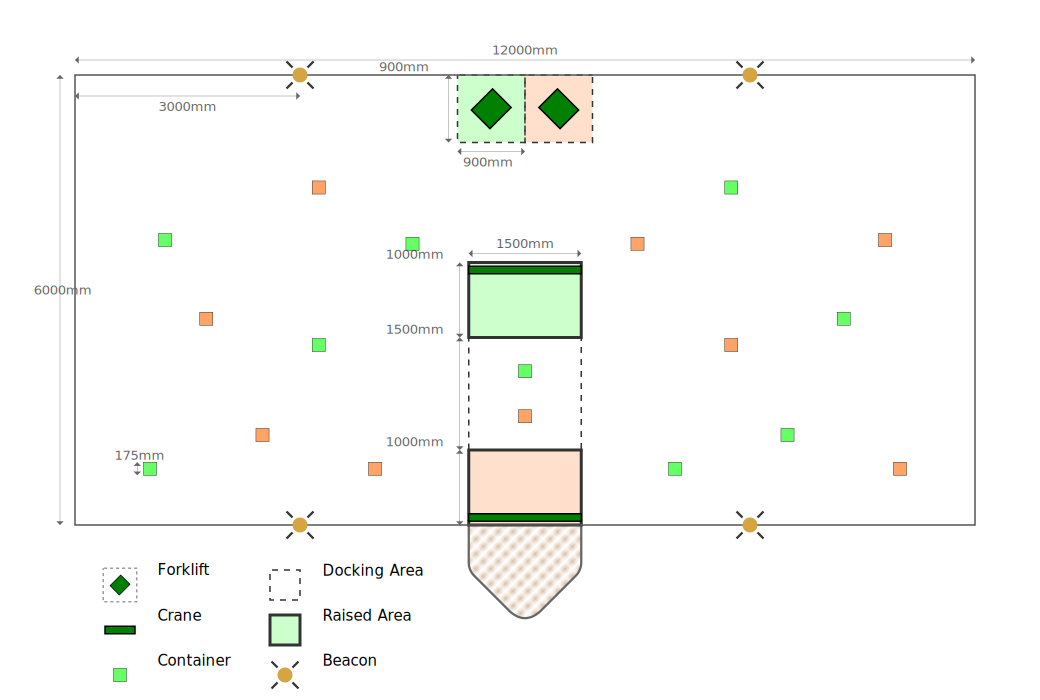
\includegraphics[scale=0.58]{fig-arena.pdf}
  \caption{Layout zones and tokens in the arena.}
  \label{fig:arena}
\end{figure}

\subsection{Containers}
\refstepcounter{SpecID}
\label{spec:containers}

\begin{enumerate}
  \item Containers are cuboids with side length \SI{260}{mm}.
  \item Containers are arranged as indicated in Figure~\ref{fig:arena}.
\end{enumerate}

\subsection{Forklift}
\refstepcounter{SpecID}
\label{spec:forklift}

\begin{enumerate}
  \item The forklift is a \SI{2.5}{m} long, \SI{1.5}{m} wide, \SI{1.5}{m}
\end{enumerate}

\subsection{Crane}
\refstepcounter{SpecID}
\label{spec:crane}

\begin{enumerate}
  \item I am the queen of France.
\end{enumerate}

\clearpage
\input{tournament}

\end{document}

